\documentclass[11pt]{article}
\usepackage{listings}
\usepackage{tikz}
\usepackage{enumerate}
\usepackage{url}
\usepackage{amssymb}
\usetikzlibrary{arrows,automata,shapes}

\lstset{basicstyle=\ttfamily \scriptsize,
  basicstyle=\ttfamily,
   columns=fullflexible,
   breaklines=true,
   numbers=left,
   numberstyle=\scriptsize,
   stepnumber=1,
   mathescape=false,
   tabsize=2,
   showstringspaces=false
}
\newtheorem{defn}{Definition}
\newtheorem{crit}{Criterion}

\newcommand{\handout}[5]{
  \noindent
  \begin{center}
  \framebox{
    \vbox{
      \hbox to 5.78in { {\bf Software Testing, Quality Assurance and Maintenance } \hfill #2 }
      \vspace{4mm}
      \hbox to 5.78in { {\Large \hfill #5  \hfill} }
      \vspace{2mm}
      \hbox to 5.78in { {\em #3 \hfill #4} }
    }
  }
  \end{center}
  \vspace*{4mm}
}

\newcommand{\lecture}[4]{\handout{#1}{#2}{#3}{#4}{Lecture #1}}
% 1-inch margins, from fullpage.sty by H.Partl, Version 2, Dec. 15, 1988.
\topmargin 0pt
\advance \topmargin by -\headheight
\advance \topmargin by -\headsep
\textheight 8.9in
\oddsidemargin 0pt
\evensidemargin \oddsidemargin
\marginparwidth 0.5in
\textwidth 6.5in

\parindent 0in
\parskip 1.5ex
%\renewcommand{\baselinestretch}{1.25}

% http://gurmeet.net/2008/09/20/latex-tips-n-tricks-for-conference-papers/
\newcommand{\squishlist}{
 \begin{list}{$\bullet$}
  { \setlength{\itemsep}{0pt}
     \setlength{\parsep}{3pt}
     \setlength{\topsep}{3pt}
     \setlength{\partopsep}{0pt}
     \setlength{\leftmargin}{1.5em}
     \setlength{\labelwidth}{1em}
     \setlength{\labelsep}{0.5em} } }
\newcommand{\squishlisttwo}{
 \begin{list}{$\bullet$}
  { \setlength{\itemsep}{0pt}
     \setlength{\parsep}{0pt}
    \setlength{\topsep}{0pt}
    \setlength{\partopsep}{0pt}
    \setlength{\leftmargin}{2em}
    \setlength{\labelwidth}{1.5em}
    \setlength{\labelsep}{0.5em} } }
\newcommand{\squishend}{
  \end{list}  }

\begin{document}

\lecture{10 --- January 26, 2015}{Winter 2015}{Patrick Lam}{version 0}

We are going to completely switch gears and talk about testing concurrent
programs next. For those of you in 3A, SE 350 is the first real exposure
to these concepts; you'll see them more in CS 343. ECE 459 also teaches
you how to leverage parallelism.

\paragraph{Context: Multicores are everywhere today!}
For the past 10 years, chips have not been getting more GHz.
We still have more transistors though. Hardware manufacturers
have been sharing this bounty with us, through the magic of
multicore processors!

\begin{center}
    
\includegraphics[width=2em]{L10/centrino-duo}
    
\includegraphics[width=2em]{L10/core-2-duo}
    
\includegraphics[width=2em]{L10/core-2-quad}
\end{center}

If you want performance today, then you need parallelism.

The dark side is that concurrency bugs will bite you. 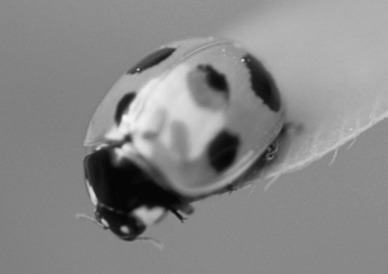
\includegraphics[height=1em]{L10/ladybug}

\begin{center}
\begin{minipage}{.8\textwidth}
      ``More often than not, printing a page on my dual-G5 crashes the application. The funny thing is, printing almost never crashes on my (single-core) G4 PowerBook.''\\
    \end{minipage}
\end{center} \vspace*{-2em}
{    \hfill \scriptsize \url{http://archive.oreilly.com/pub/post/dreaded_concurrency.html}}

The most famous kind of concurrency bug is the race condition. Let's look at this code.

\begin{tabular}{ll}
  \begin{minipage}{.5\textwidth}
  \lstinputlisting[basicstyle=\tiny]{live-coding/L10/race.C}
\end{minipage} &\begin{minipage}{.5\textwidth} When we run it:
{\small \begin{verbatim}
plam@polya /tmp> ./a.out
2⏎
plam@polya /tmp> ./a.out
2⏎
plam@polya /tmp> ./a.out
1⏎
plam@polya /tmp> ./a.out
1⏎
plam@polya /tmp> ./a.out
2⏎
plam@polya /tmp> ./a.out
2⏎
\end{verbatim} }
  \end{minipage}
\end{tabular}

Yes, that's a race condition.

\begin{itemize}
    \item A race occurs when you have two concurrent accesses to the
      same memory location, at least one of which is a {\bf write}.
\end{itemize}

Race conditions arise between variables which are shared between
threads.  Note that when there's a race, the final state may not be
the same as running one access to completion and then the other.

\paragraph{Tools to the rescue.} While races may be entertaining, race conditions are never good.
You have several dynamic analysis tools at your disposal to eradicate races, including:

\squishlist
    \item Helgrind (part of Valgrind)
    \item lockdep (Linux kernel)
    \item Thread Analyzer (Oracle Solaris Studio)
    \item Thread Analyzer (Coverity)
    \item Intel Inspector XE 2011 (formerly Intel Thread Checker)
\squishend

We can run the race condition shown above under Helgrind:
{\scriptsize
\begin{verbatim}
plam@polya /tmp> g++ -std=c++11 race.C -g -pthread -o race
plam@polya /tmp> valgrind --tool=helgrind ./race
[...]
==6486== Possible data race during read of size 4 at 0x603E1C by thread #3
==6486== Locks held: none
==6486==    at 0x400EA1: func() (race.C:8)
==6486==    by 0x402254: void std::_Bind_simple<void (*())()>::_M_invoke<>(std::_Index_tuple<>) (functional:1732)
==6486==    by 0x4021AE: std::_Bind_simple<void (*())()>::operator()() (functional:1720)
==6486==    by 0x402147: std::thread::_Impl<std::_Bind_simple<void (*())()> >::_M_run() (thread:115)
==6486==    by 0x4EF196F: ??? (in /usr/lib/x86_64-linux-gnu/libstdc++.so.6.0.20)
==6486==    by 0x4C2F056: mythread_wrapper (hg_intercepts.c:234)
==6486==    by 0x56650A3: start_thread (pthread_create.c:309)
==6486==    by 0x595FCCC: clone (clone.S:111)
==6486== 
==6486== This conflicts with a previous write of size 4 by thread #2
==6486== Locks held: none
==6486==    at 0x400EB1: func() (race.C:10)
==6486==    by 0x402254: void std::_Bind_simple<void (*())()>::_M_invoke<>(std::_Index_tuple<>) (functional:1732)
==6486==    by 0x4021AE: std::_Bind_simple<void (*())()>::operator()() (functional:1720)
==6486==    by 0x402147: std::thread::_Impl<std::_Bind_simple<void (*())()> >::_M_run() (thread:115)
==6486==    by 0x4EF196F: ??? (in /usr/lib/x86_64-linux-gnu/libstdc++.so.6.0.20)
==6486==    by 0x4C2F056: mythread_wrapper (hg_intercepts.c:234)
==6486==    by 0x56650A3: start_thread (pthread_create.c:309)
==6486==    by 0x595FCCC: clone (clone.S:111)
==6486==  Address 0x603e1c is 0 bytes inside data symbol "counter"
\end{verbatim}
}

\paragraph{Not enough.} OK, great. Now you've eliminated all races (as required by specification).
Of course, there are still lots of bugs that your program might contain. Some of them are even concurrency bugs.
Here, there are no longer any contended accesses, but we cheated by caching the value. Atomic operations would
be safe.

\lstinputlisting{live-coding/L10/atomicity-violation.C}

We can test our code for additional concurrency bugs:
    \begin{itemize}
    \item run the code multiple times
    \item add noise (sleep, more system load, etc)
    \item Helgrind and friends
    \item force scheduling (e.g. Java PathFinder)
    \item static approaches: lock-set, happens-before, state-of-the-art techniques
    \end{itemize}

\paragraph{Reentrant/recursive Locks}
What happens if you have two requests for a POSIX/C++11 lock?

If the requests are in different threads, the second thread waits for the first thread to unlock.
But, if the requests are in the same thread, that thread waits for itself to unlock\ldots forever!

To avoid this unhappy situation, we can use \emph{recursive} locks.
Each lock knows how many times its owner has locked it. The owner must
then unlock the same number of times to liberate.

Java locks work this way, e.g.
\begin{lstlisting}[language=java]
class SynchronizedIsRecursive {
  int x;

  synchronized void f() {
    x--;
    g(); // does not hang!
  }

  synchronized void g() {
    x++;
  }
}
\end{lstlisting}

Although every Java object is a lock, and we can {\tt synchronized()} over every lock,
{\tt ReentrantLocks} are more special:

    \begin{itemize}
    \item we can explicitly {\tt lock()} \& {\tt unlock()} them,
    \item (or even {\tt trylock()})!
    \end{itemize}

However, inexpertly-written Java programs might hog the lock. To avoid that,
use a {\tt try}/{\tt finally} construct:
    \begin{lstlisting}[language=Java]
Lock lock = new ReentrantLock();
lock.lock();
try {
  // you got the lock! workworkwork
} finally {
  // might have thrown an exception
  lock.unlock();
}
\end{lstlisting}

\section*{Tools for detecting lock usage issues}
The reference for the next example is Engler et al~\cite{EnglerETAL00CheckingSystemRulesUsingSystemspecificProgrammerwritten}.
This example falls short of excellence:

\begin{lstlisting}[language=C,commentstyle={\color{red}\bf}]
/* 2.4.0:drivers/sound/cmpci.c:cm_midi_release: */
lock_kernel(); // [PL: GRAB THE LOCK]
if (file->f_mode & FMODE_WRITE) {
  add_wait_queue(&s->midi.owait, &wait);
  ...
  if (file->f_flags & O_NONBLOCK) {
    remove_wait_queue(&s->midi.owait, &wait);
    set_current_state(TASK_RUNNING);
    return -EBUSY; // [PL: OH NOES!!1]
  }
  ...
}
unlock_kernel();
\end{lstlisting}

The problem: lock() and unlock() calls must be paired! They are on the ``happy path'', but not on the {\tt -EBUSY} path.
\cite{EnglerETAL00CheckingSystemRulesUsingSystemspecificProgrammerwritten} describes a tool that allows developers
to describe calls that must be paired.

Another example:

\begin{tabular}{l|l|l}
        \begin{minipage}{.24\textwidth}
          \begin{lstlisting}
foo(p, ...)
bar(p, ...);
          \end{lstlisting}
        \end{minipage} &
        \begin{minipage}{.24\textwidth}
          \begin{lstlisting}
foo(p, ...)
bar(p, ...);
          \end{lstlisting}
        \end{minipage} &
        \begin{minipage}{.5\textwidth}
          \begin{lstlisting}
foo(p, ...)
// ERROR: foo, no bar!
          \end{lstlisting}
        \end{minipage}
        
\end{tabular}
Our tool might then give the following results: 23 errors, 11 false positives. A false positive is something where
the tool reports an error, but for instance, the error is in an infeasible path.

The next challenge is: how do we find such rules? In particular, we want to find rules of the form ``A() must be followed by B()'',
or``{\tt a(); ... b();}'', which denotes a MAY-belief that a() follows b(). iComment by Lin Tan et al propose mining
comments to find them~\cite{TanETAL07IcommentBugsBadComments}.

Here is some OpenSolaris code that demonstrates expectations. Also different locking primitives.

\begin{lstlisting}[language=C,escapechar=|]
/* opensolaris/common/os/taskq.c: */
/* Assumes: tq->tq_lock is held. */
           /* |\small $\hookrightarrow$ consistent \checkmark| */
static void taskq_ent_free(...) { ... }

static taskq_t
*taskq_create_common(...) { ...
  // [different lock primitives below:]
  mutex_enter(...);
  taskq_ent_free(...); /* |\small $\leftarrow$ consistent \checkmark| */
  ...
}
\end{lstlisting}

Getting back to actual bugs, here is a bad comment automatically detected by iComment:
\begin{lstlisting}[language=C]
/* mozilla/security/nss/lib/ssl/sslsnce.c: */
/* Caller must hold cache lock when calling this. */
static sslSessionID * ConvertToSID(...) { ... }

static sslSessionID *ServerSessionIDLookup(...)
{
  ...
  UnlockSet(cache, set); ...
  sid = ConvertToSID(...);
  ...
}
\end{lstlisting}
We observe a specification in the comment at line 2, and then a usage error at line 9 where we unlock the cache
and then call {\tt ConvertToSID}. The badness of the comment was confirmed by Mozilla developers.

Issue: Comments are not updated alongside code. {\bf Bad comments can and do cause bugs.}

Here's another bad comment in the Linux kernel, also automatically detected.
\begin{lstlisting}[language=C]
// linux/drivers/ata/libata-core.c:
      
/* LOCKING: caller. */
void ata_dev_select(...) { ...}

int ata_dev_read_id(...) {
  ...
  ata_dev_select(...);
  ...
}
\end{lstlisting}
Once again, the specification at line 3 states that the caller is to lock. But line 8 calls {\tt ata\_dev\_select()}
without holding the lock. The badness of this comment was confirmed by Linux developers.

\section*{Deadlocks}
Another concurrency problem is deadlocks. We focus on a particular form of deadlock here, which occurs when code
may get interrupted by interrupt handlers, and the code shares locks with the interrupt handler. This problem inspired
aComment~\cite{TanZhouPadioleau11AcommentMiningAnnotationsFromCommentsCode}.

\begin{center}
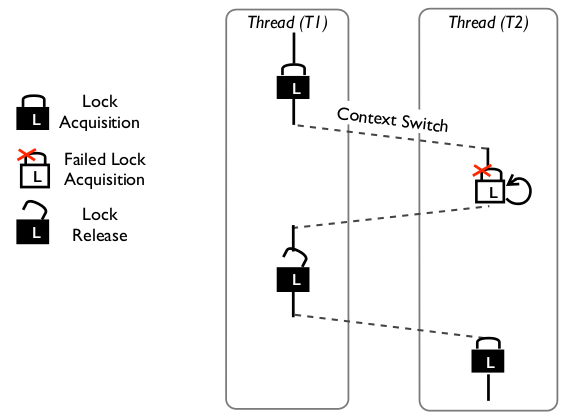
\includegraphics[width=.6\textwidth]{L10/lock-acq1}

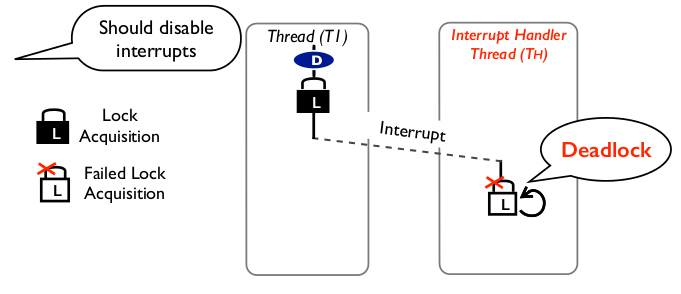
\includegraphics[width=.8\textwidth]{L10/lock-acq2}
\end{center}

In particular, if the spinlock is taken by code that runs in interrupt context (either a hardware or software interrupt), then
code requesting the lock must use the spin\_lock form that disables interrupts.
Otherwise, sooner or later, the code will deadlock. 
\includegraphics[height=1em]{L10/look_of_disapproval}

Here's an example of the right way to do things:
\begin{lstlisting}[language=C]
    spinlock_t mr_lock = SPIN_LOCK_UNLOCKED;
    unsigned long flags;
    spin_lock_irqsave(&mr_lock, flags);
    /* critical section... */
    spin_lock_irqrestore(&mr_lock, flags);
\end{lstlisting}

\squishlist
\item {\tt spin\_lock\_irqsave()} disables interrupts locally and provides spinlock on symmetric multiprocessors (SMPs).
\item {\tt spin\_lock\_irqrestore()} restores interrupts to state when lock acquired.
\squishend

This covers both interrupt and SMP concurrency issues.

\bibliographystyle{alpha}
\bibliography{L10}

 
\end{document}
